\documentclass{beamer}

\usepackage[T1]{fontenc}
\usepackage[utf8]{inputenc}
\usepackage[french]{babel}
\usepackage{amsmath,amsthm}
\usepackage{amssymb,cmll}
\usepackage{ebproof}
\usepackage{mathtools}
\usepackage{hyperref}
\usepackage{tikz}
\usetikzlibrary{trees}
\usepackage{bm}
\usepackage{algorithm}
\floatname{algorithm}{Algorithme}
\usepackage{algpseudocode}
\usepackage{hyperref}
\usepackage{minted}
\usepackage{authblk}
\usepackage[backend=biber,style=alphabetic,sorting=ynt]{biblatex}
\usepackage[export]{adjustbox}

% dessins arbres : tikz
\tikzset{baseline=(current bounding box.center)}
\tikzset{level distance=1.3cm}

%imported from click and collect
\newcommand*{\orth}{^\perp}
\newcommand*{\tensor}{\otimes}

\newcommand*{\namedproofv}[2]{\hypo{#1}\infer[no rule]{1}{\vdash #2}}
\newcommand*{\hypv}[1]{\hypo{\vdash #1}}
\newcommand*{\axv}[1]{\infer{0}[\ensuremath{\mathit{ax}}]{\vdash #1}}
\newcommand*{\cutv}[1]{\infer{2}[\ensuremath{\mathit{cut}}]{\vdash #1}}
\newcommand*{\onev}[1]{\infer{0}[\ensuremath{\one}]{\vdash #1}}
\newcommand*{\botv}[1]{\infer{1}[\ensuremath{\bot}]{\vdash #1}}
\newcommand*{\topv}[1]{\infer{0}[\ensuremath{\top}]{\vdash #1}}
\newcommand*{\tensorv}[1]{\infer{2}[\ensuremath{\tensor}]{\vdash #1}}
\newcommand*{\parrv}[1]{\infer{1}[\ensuremath{\parr}]{\vdash #1}}
\newcommand*{\permv}[2]{\infer{1}[\ensuremath{\textit{ex}_{#1}}]{\vdash #2}}
\newcommand*{\withv}[1]{\infer{2}[\ensuremath{\with}]{\vdash #1}}
\newcommand*{\pluslv}[1]{\infer{1}[\ensuremath{\plus_1}]{\vdash #1}}
\newcommand*{\plusrv}[1]{\infer{1}[\ensuremath{\plus_2}]{\vdash #1}}
\newcommand*{\ocv}[1]{\infer{1}[\ensuremath{\oc}]{\vdash #1}}
\newcommand*{\wkv}[1]{\infer{1}[\ensuremath{?\mathit{w}}]{\vdash #1}}
\newcommand*{\cov}[1]{\infer{1}[\ensuremath{?\mathit{c}}]{\vdash #1}}
\newcommand*{\dev}[1]{\infer{1}[\ensuremath{?\mathit{d}}]{\vdash #1}}
\newcommand*{\defv}[1]{\infer[dashed]{1}[\ensuremath{\mathit{def}}]{\vdash #1}}
\newcommand*{\permapp}[2]{#2 #1}
\newcommand*{\someperm}{\varsigma}
\newcommand*{\someadd}{\rho}
\newcommand*{\someaddbis}{w}
\newcommand*{\someproof}{\pi}
\newcommand*{\sequent}{\Gamma}
\newcommand*{\sequentbis}{\Delta}
\newcommand*{\size}[1]{\mathopen{|}#1\mathclose{|}}

\newcommand*{\Left}{\textnormal{\texttt{L}}}
\newcommand*{\Right}{\textnormal{\texttt{R}}}

\newcommand*{\proofs}{\ensuremath{\mathcal{P}}}
\newcommand*{\sequents}{\ensuremath{\mathcal{S}}}
\newcommand*{\addresses}{\ensuremath{\mathcal{A}}}
\newcommand*{\treeaddresses}{\ensuremath{\mathcal{A'}}}
\newcommand*{\trees}{\ensuremath{\mathcal{T}}}
\newcommand*{\treespartial}{\ensuremath{\mathcal{T'}}}
\newcommand*{\representationslarge}{\ensuremath{\trees \times \sequents}}
\newcommand*{\representations}{\ensuremath{\mathcal{R}}}
\newcommand*{\representationspartiallarge}{\ensuremath{\treespartial \times \sequents}}
\newcommand*{\representationspartial}{\ensuremath{\mathcal{R'}}}
\newcommand*{\setshuffle}{\bowtie}

\newcommand*{\encode}{\ensuremath{\varphi}}
\newcommand*{\decode}{\ensuremath{\gamma}}

\newcommand*{\height}{\ensuremath{h}}
\newcommand*{\relapprox}{\ensuremath{\triangleleft}}
\newcommand*{\relapproxlarge}{\ensuremath{\relapprox^*}}
\newcommand*{\unknown}{H}

\newcommand*{\lowapprox}{\ensuremath{\Sigma_0}}
\newcommand*{\lowapproxspec}{\ensuremath{\Sigma'_0}}
\newcommand*{\highapprox}{\ensuremath{\Sigma_1}}
\newcommand*{\highapproxspec}{\ensuremath{\Sigma'_1}}

\newcommand*{\foblig}[1]{\textcolor{red}{#1}}

\newcommand*{\treesimplify}{\ensuremath{s}}

\newcommand*{\caddpartial}{(a)}
\newcommand*{\clinpartial}{(b')}
\newcommand*{\cdespartial}{(c)}

\newcommand*{\exactcond}{\bigstar_1}
\newcommand*{\exactcondbis}{\bigstar_2}

\title{Conception et implémentation d'un assistant de preuve pour le fragment multiplicatif de la logique linéaire}
\author{Jonas Torriero-Meskour}
\institute{ENS de Lyon, stage de L3 au LIP encadré par Olivier Laurent}
\date{4 juin 2024 -- 19 juillet 2024}

\addtobeamertemplate{navigation symbols}{}{ \hspace{1em}    \usebeamerfont{footline}%
    \insertframenumber / \inserttotalframenumber }

\begin{document}

\begin{frame}
   \titlepage
\end{frame}

\begin{frame}{Plan général}
    \begin{itemize}
        \item Introduction \& objectif du stage
            \pause
        \item Présentation de la logique linéaire
            \pause
        \item Principe général de l'assistant de preuve
            \pause
        \item Quelques résultats de fiabilité
            \pause
        \item Conclusion
    \end{itemize}
\end{frame}

\begin{frame}{Introduction}
    \begin{itemize}
        \item Logique linéaire: introduite en 1987 par Jean-Yves Girard.
            \pause
        \item On s'intéresse au fragment multiplicatif MLL.
            \pause
        \item Intérêt: voir les hypothèses comme des ressources.
            \pause
        \item Nombreuses applications en informatique: programmation fonctionnelle, théorie de la preuve...
            \pause
        \item D'où une nécessité... écrire facilement des preuves!
    \end{itemize}    
\end{frame}

\begin{frame}{Problématique}
    \begin{itemize}
        \item Plusieurs syntaxes possibles, dont... le calcul des séquents!
            \pause
        \item Notre objectif: concevoir un assitant de preuve interactif pour le calcul des séquents, guidant l'utilisateur efficacement et pas à pas.
    \end{itemize}
\end{frame}

\begin{frame}{Un prédecesseur}
    \centering
    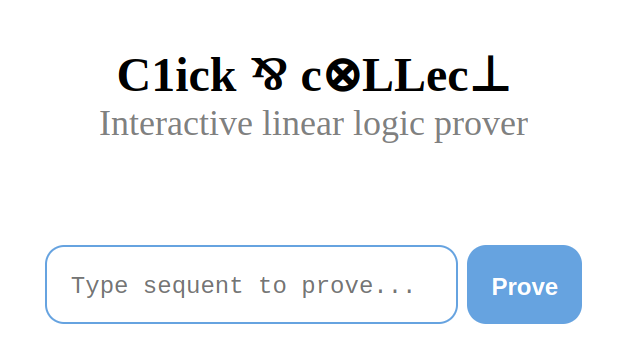
\includegraphics[scale=0.35]{images/C&C_home.png}

    \pause
    
    \begin{itemize}
        \item L'une des premières interfaces graphiques pour le calcul des séquents linéaire.
            \pause
        \item Cependant... but pédagogique, s'adresse à des débutants.
            \pause
        \item Problème: inadapté à utilisateur expert, l'information demandée est redondante.
    \end{itemize}

%%démo? ou après "La structure des preuves est redondante"

\end{frame}

\begin{frame}{Objectif du stage}
    \begin{itemize}
        \item Concevoir un outil pour les utilisateurs experts.
            \pause
        \item Notre contribution:
            \begin{itemize}
                \item Travailler sur un formalisme du calcul des séquents éliminant les redondances.
                
                \item Concevoir une interface interactive automatisant certains choix, et minimisant l'information requise par ailleurs.
            \end{itemize}
            \pause
        \item Résultat: mll\_prover, implémenté en OCaml !
    \end{itemize}
\end{frame}

\begin{frame}{Séquents en logique linéaire}
    \begin{itemize}
        \item Formules: $F := X \mid X\orth \mid F \parr F \mid F \tensor F$.
            \pause
        \item Intuition: $\orth \sim \neg$, $\parr \sim \lor$, $\tensor \sim \land$.
            \pause
        \item Remarque: on ne peut nier que les atomes.
            \pause \\ 
        \item Les séquents sont unilatéraux: en logique classique, \\ $A \vdash B$ $\; \sim \; \; \vdash A \implies B$ $\; \sim \; \; \vdash \neg A \lor B$.\\         \pause
        \item Séquent: liste de formules. Un séquent est intuitivement une disjonction: $\vdash X_1, X_2, X_3$ $\sim \; \vdash X_1 \lor X_2 \lor X_3$. 
        \pause\\
        $\rightarrow$ En logique linéaire: $\vdash A\orth{}, B$.
    \end{itemize}
\end{frame}

\begin{frame}{Quelques exemples de séquents}
    \begin{itemize}
        \item $F := X \mid X\orth \mid F \parr F \mid F \tensor F$.\\
        $\orth \sim \neg$, $\parr \sim \lor$, $\tensor \sim \land$.\\
        Séquent: liste de formules (intuitivement leur disjonction).
            \pause
        \item $X\orth{}, X$ $\; \sim \; \neg X \lor X$. \\
        \pause $\rightarrow$ C'est une tautologie!
            \pause
        \item $A, B \tensor C$ $\; \sim \; A \lor (B \land C)$.
            \pause
        \item $A,B \parr C\orth{}$ $\; \sim \; A \lor B \lor \neg C$ $\; \sim \; A, B, C\orth{}$. \\
        \pause $\rightarrow$ Utilité du par?
            \pause
        \item Formules imbriquées:\\
        \pause $(A \parr B) \tensor C$ $\; \sim \; (A \lor B) \land C$.
    \end{itemize}
\end{frame}

\begin{frame}{Preuves en calcul des séquents linéaire}
    \begin{itemize}
        \item L'ensemble des preuves \proofs{} est défini par les règles d'induction suivantes:\pause
            \begin{equation*}
            \begin{prooftree}
              \axv{X\orth, X}
            \end{prooftree}
            \; \; \;
            \begin{prooftree}
              \hypv{\sequent}
              \permv{\someperm}{\permapp{\someperm}{\sequent}}
            \end{prooftree}
            \; \; \;
            \begin{prooftree}
              \hypv{\sequent, A, B, \sequentbis}
              \parrv{\sequent, A \parr B, \sequentbis}
            \end{prooftree}
            \; \; \;
            \begin{prooftree}
              \hypv{\sequent, A}
              \hypv{B, \sequentbis}
              \tensorv{\sequent, A \tensor B, \sequentbis}
            \end{prooftree}
            \end{equation*}
            \pause
        \item Règle $\textit{ex}_{\someperm}$: les séquents sont des \textit{multi-ensembles} (où l'on distingue les occurences), réalisés par des \textit{listes}.
            \pause
        \item Règle $\tensor$: introduit la notion de coût sur les hypothèses.\\
        \pause Prouver $A \tensor B$ revient à prouver $A$ et $B$. Pour prouver $A \tensor B$ à partir d'un ensemble d'hypothèses $\Sigma$, on doit en choisir une partition $\sequent, \sequentbis$, et prouver $A$ avec toutes les hypothèses de $\sequent$, et $B$ avec toutes celles de $\sequentbis$.
    \end{itemize}
\end{frame}

\begin{frame}{Exemple: une preuve où l'on choisit la partition}
    \begin{itemize}
        \item Règles: 
            \begin{equation*}
            \begin{prooftree}
              \axv{X\orth, X}
            \end{prooftree}
            \; \; \;
            \begin{prooftree}
              \hypv{\sequent}
              \permv{\someperm}{\permapp{\someperm}{\sequent}}
            \end{prooftree}
            \; \; \;
            \begin{prooftree}
              \hypv{\sequent, A, B, \sequentbis}
              \parrv{\sequent, A \parr B, \sequentbis}
            \end{prooftree}
            \; \; \;
            \begin{prooftree}
              \hypv{\sequent, A}
              \hypv{B, \sequentbis}
              \tensorv{\sequent, A \tensor B, \sequentbis}
            \end{prooftree}
            \end{equation*}
        \item On partitionne $\Sigma = \{{X_1}\orth, {X_2}\orth\}$:
        \begin{equation*}
        \begin{prooftree}
            \axv{{X_1}\orth, X_1}
            \axv{{X_2}\orth, X_2}
            \permv{(2, 1)}{X_2, {X_2}\orth}
            \tensorv{{X_1}\orth, X_1 \tensor X_2, {X_2}\orth}
            \permv{(3, 2, 1)}{{X_2}\orth, X_1 \tensor X_2, {X_1}\orth}
        \end{prooftree}
        \end{equation*}
    \end{itemize}
\end{frame}

\begin{frame}{La structure des preuves est redondante}
    \begin{itemize}
        \item L'information nécessaire est en rouge:
            \begin{equation*}
            \begin{prooftree}
                \hypv{X_1, {X_1}\orth, X_2, {X_2}\orth}
                {\infer{1}[\foblig{\ensuremath{\parr}}]{\vdash \foblig{X_1, {X_1}\orth \parr X_2, {X_2}\orth}}}
            \end{prooftree}
            \end{equation*}
            \pause
        \item En fait, les permutations ne sont jamais nécessaires:
            \begin{equation*}
                \begin{prooftree}
                    \axv{\foblig{{X_1}\orth, X_1}}
                    \axv{\foblig{{X_2}\orth, X_2}}
                    \permv{(2, 1)}{X_2, {X_2}\orth}
                    {\infer{2}[\foblig{\ensuremath{\tensor}}]{{X_1}\orth, X_1 \mathbin{\foblig{\tensor}} X_2, {X_2}\orth}}
                    \permv{(3, 2, 1)}{\foblig{{X_2}\orth, X_1 \tensor X_2, {X_1}\orth}}
                \end{prooftree}
            \end{equation*}
    \end{itemize}
\end{frame}

\begin{frame}{Cette redondance se retrouve dans Click \& Collect}
    \begin{center}
        \adjincludegraphics[height=5.5cm,trim={{.25\width} {.35\height} {.25\width} {.15\height}},clip]{images/C&C_demo1.png}
    \end{center}
\end{frame}

\begin{frame}{Cette redondance se retrouve dans Click \& Collect}
    \begin{center}
        \adjincludegraphics[height=5.5cm,trim={{.25\width} {.35\height} {.25\width} {.15\height}},clip]{images/C&C_demo2.png}
    \end{center}
\end{frame}

\begin{frame}{Cette redondance se retrouve dans Click \& Collect}
    \begin{center}
        \adjincludegraphics[height=5.5cm,trim={{.25\width} {.30\height} {.25\width} {.15\height}},clip]{images/C&C_demo3.png}
    \end{center}
\end{frame}

\begin{frame}{Cette redondance se retrouve dans Click \& Collect}
    \begin{center}
        \adjincludegraphics[height=5.5cm,trim={{.25\width} {.30\height} {.25\width} {.15\height}},clip]{images/C&C_demo4.png}
    \end{center}
\end{frame}

\begin{frame}{Cette redondance se retrouve dans Click \& Collect}
    \begin{center}
        \adjincludegraphics[height=5.5cm,trim={{.25\width} {.30\height} {.25\width} {.15\height}},clip]{images/C&C_demo5.png}
    \end{center}
\end{frame}

\begin{frame}{Notre solution}
    \begin{itemize}
        \item Manipuler en arrière-plan des représentations non-redondantes, équivalentes aux preuves.
            \pause
        \item Utiliser des heuristiques d'autocomplétion et de détection d'erreurs.
     \end{itemize}
\end{frame}

\begin{frame}{Représentations}
    Couple $(t, \sequent)$, où $t$ est un arbre encodant le squelette de la preuve, et $\sequent$ est le séquent prouvé.
    \begin{equation*}
    \begin{prooftree}
        \axv{{X_1}\orth, X_1}
        \axv{{X_2}\orth, X_2}
        \permv{(2, 1)}{X_2, {X_2}\orth}
        \tensorv{{X_1}\orth, X_1 \tensor X_2, {X_2}\orth}
        \parrv{{X_1}\orth \parr (X_1 \tensor X_2), {X_2}\orth}
    \end{prooftree} \pause
    \end{equation*}\\
    \begin{equation*}
    \begin{tikzpicture}%
        [level 2/.style={sibling distance=3.5cm}]
        \node {$U_{1 \epsilon}$}
        child {node {$B_{1 \Right}$}
            child {node {$F_{1 \Left, \; 1 \Right \cdot \Left}$}}
            child {node {$F_{1 \Right \cdot \Right, \; 2 \epsilon}$}}
        };
    \end{tikzpicture}\vdash {X_1}\orth \parr (X_1 \tensor X_2), {X_2}\orth
    \end{equation*}
%%couleurs pour relier éléments en calcul des séquents et dans l'arbre (adresses notamment)
\end{frame}

%% ajouter théorèmes d'équivalence

\begin{frame}{Représentations partielles}
    \begin{itemize}
        \item On étend nos représentations à des représentations partielles.
            \pause
        \item Elles ont des ``trous'', correspondant aux endroits de la preuve qu'on ne connaît pas encore.
            \pause
        \item Exemple:
            \begin{equation*}
                \begin{tikzpicture}%
                    [level 2/.style={sibling distance=3.5cm}]
                    \node {$U_{3 \epsilon}$}
                    child {node {$B_{1 \epsilon}$}
                        child {node {$\unknown$}}
                        child {node {$\unknown$}}
                    };
                \end{tikzpicture}
                \vdash X_1\tensor X_2\orth, X_2\tensor X_3\orth, X_1\orth\parr X_3
            \end{equation*}
            \begin{prooftree*}
                  \hypv{X_1, X_2\tensor X_3\orth, X_1\orth, X_3}
                  \hypv{X_2\orth, X_2\tensor X_3\orth, X_1\orth, X_3}
               \tensorv{X_1\tensor X_2\orth, X_2\tensor X_3\orth, X_1\orth, X_3}
            \parrv{X_1\tensor X_2\orth, X_2\tensor X_3\orth, X_1\orth\parr X_3}
            \end{prooftree*}
    \end{itemize}
\end{frame}

\begin{frame}{Principe général de l'assistant}
    \begin{itemize}
        \item L'utilisateur donne un séquent $\sequent$ à prouver, et part de la représentation partielle minimale $(\unknown, \sequent)$.
            \pause
        \item Guidé par l'assisant, il colmate étape par étape les trous, en les remplaçant par des informations sur la preuve.
            \pause
        \item S'il aboutit à une représentation complète, elle est décodée et la preuve est affichée.
    \end{itemize}
\end{frame}

\begin{frame}{Un exemple d'exécution}
    L'utilisateur veut prouver ${X_1}\orth \parr (X_1 \tensor X_2), {X_2}\orth$:
        \pause \\
    \begin{equation*}
    \pause
    \unknown 
    \pause
    \relapprox
    \begin{tikzpicture}%
        [level 2/.style={sibling distance=3.5cm}]
        \node {$U_{1 \epsilon}$}
        child {node {$\unknown$}
        };
    \end{tikzpicture}
    \pause
    \relapprox
    \begin{tikzpicture}%
        [level 2/.style={sibling distance=1.5cm}]
        \node {$U_{1 \epsilon}$}
        child {node {$B_{1 \Right}$}
            child {node {$\unknown$}}
            child {node {$\unknown$}}
        };
    \end{tikzpicture}
    \pause
    \relapprox
    \begin{tikzpicture}%
        [level 2/.style={sibling distance=1.5cm}]
        \node {$U_{1 \epsilon}$}
        child {node {$B_{1 \Right}$}
            child {node {$F_{1 \Left, \; 1 \Right \cdot \Left}$}}
            child {node {$\unknown$}}
        };
    \end{tikzpicture}
    \pause
    \relapprox
    \begin{tikzpicture}%
        [level 2/.style={sibling distance=1.5cm}]
        \node {$U_{1 \epsilon}$}
        child {node {$B_{1 \Right}$}
            child {node {$F_{1 \Left, \; 1 \Right \cdot \Left}$}}
            child {node {$F_{1 \Right \cdot \Right, \; 2 \epsilon}$}}
        };
    \end{tikzpicture}
    \end{equation*}
\end{frame}

\begin{frame}{Un exemple d'exécution}
    La construction a abouti à une représentation complète:
    \begin{equation*}
        \begin{tikzpicture}%
            [level 2/.style={sibling distance=3.5cm}]
            \node {$U_{1 \epsilon}$}
            child {node {$B_{1 \Right}$}
                child {node {$F_{1 \Left, \; 1 \Right \cdot \Left}$}}
                child {node {$F_{1 \Right \cdot \Right, \; 2 \epsilon}$}}
            };
        \end{tikzpicture}
        \vdash {X_1}\orth \parr (X_1 \tensor X_2), {X_2}\orth
    \end{equation*}
    \pause qu'on affiche en tant que preuve!
    \begin{equation*}
        \begin{prooftree}
            \axv{{X_1}\orth, X_1}
            \axv{{X_2}\orth, X_2}
            \permv{(2, 1)}{X_2, {X_2}\orth}
            \tensorv{{X_1}\orth, X_1 \tensor X_2, {X_2}\orth}
            \parrv{{X_1}\orth \parr (X_1 \tensor X_2), {X_2}\orth}
        \end{prooftree}
    \end{equation*}
\end{frame}

\begin{frame}{Fiabilité de l'assistant}
    \begin{itemize}
        \item Correction: \pause si l'utilisateur aboutit, le guidage de notre assistant assure que la preuve construite est correcte.
            \pause
        \item Complétude: à permutations intermédiaires près, il est possible de construire n'importe quelle preuve grâce à notre assistant.
            \pause
        \item Les heuristiques d'autocomplétion et de détection d'erreurs sont correctes, et ne retirent pas d'expressivité à l'utilisateur.
    \end{itemize}
\end{frame}

\begin{frame}{Conclusion}
    \begin{itemize}
        \item mll\_prover est plus efficace que Click \& Collect pour les utilisateurs experts.
            \pause
        \item Par exemple: prouver $X_5, X_4, {X_1}\orth \tensor ({X_2}\orth \tensor ({X_3}\orth \tensor ({X_4}\orth \tensor {X_5}\orth))), X_1, X_3 \parr X_2$.\\
        Entre $1$ et $3$ opérations avec mll\_prover, plusieurs dizaines avec Click \& Collect.
            \pause
        \item Pistes d'améliorations:
            \begin{itemize}
                \item ajouter une interface graphique.
                \item revenir en arrière dans les choix.
                \item enrichir les heuristiques d'autocomplétion.
                \item étendre l'assistant à LL.
            \end{itemize}
    \end{itemize}
\end{frame}

\end{document}